\documentclass{standalone}
    \usepackage{tikz}
    \usepackage{pgfplots}
    \usetikzlibrary{calc}
    \usetikzlibrary{patterns}
\mathversion{bold}    
% defining the new dimensions and parameters
\newlength{\hatchspread}
\newlength{\hatchthickness}
\newlength{\hatchshift}
\newcommand{\hatchcolor}{}
% declaring the keys in tikz
\tikzset{hatchspread/.code={\setlength{\hatchspread}{#1}},
         hatchthickness/.code={\setlength{\hatchthickness}{#1}},
         hatchshift/.code={\setlength{\hatchshift}{#1}},% must be >= 0
         hatchcolor/.code={\renewcommand{\hatchcolor}{#1}}}
% setting the default values
\tikzset{hatchspread=3pt,
         hatchthickness=0.4pt,
         hatchshift=0pt,% must be >= 0
         hatchcolor=black}
% declaring the pattern
\pgfdeclarepatternformonly[\hatchspread,\hatchthickness,\hatchshift,\hatchcolor]% variables
   {custom north west lines}% name
   {\pgfqpoint{\dimexpr-2\hatchthickness}{\dimexpr-2\hatchthickness}}% lower left corner
   {\pgfqpoint{\dimexpr\hatchspread+2\hatchthickness}{\dimexpr\hatchspread+2\hatchthickness}}% upper right corner
   {\pgfqpoint{\dimexpr\hatchspread}{\dimexpr\hatchspread}}% tile size
   {% shape description
    \pgfsetlinewidth{\hatchthickness}
    \pgfpathmoveto{\pgfqpoint{0pt}{\dimexpr\hatchspread+\hatchshift}}
    \pgfpathlineto{\pgfqpoint{\dimexpr\hatchspread+0.15pt+\hatchshift}{-0.15pt}}
    \ifdim \hatchshift > 0pt
      \pgfpathmoveto{\pgfqpoint{0pt}{\hatchshift}}
      \pgfpathlineto{\pgfqpoint{\dimexpr0.15pt+\hatchshift}{-0.15pt}}
    \fi
    \pgfsetstrokecolor{\hatchcolor}
%    \pgfsetdash{{1pt}{1pt}}{0pt}% dashing cannot work correctly in all situation this way
    \pgfusepath{stroke}
   }

\begin{document}
\huge
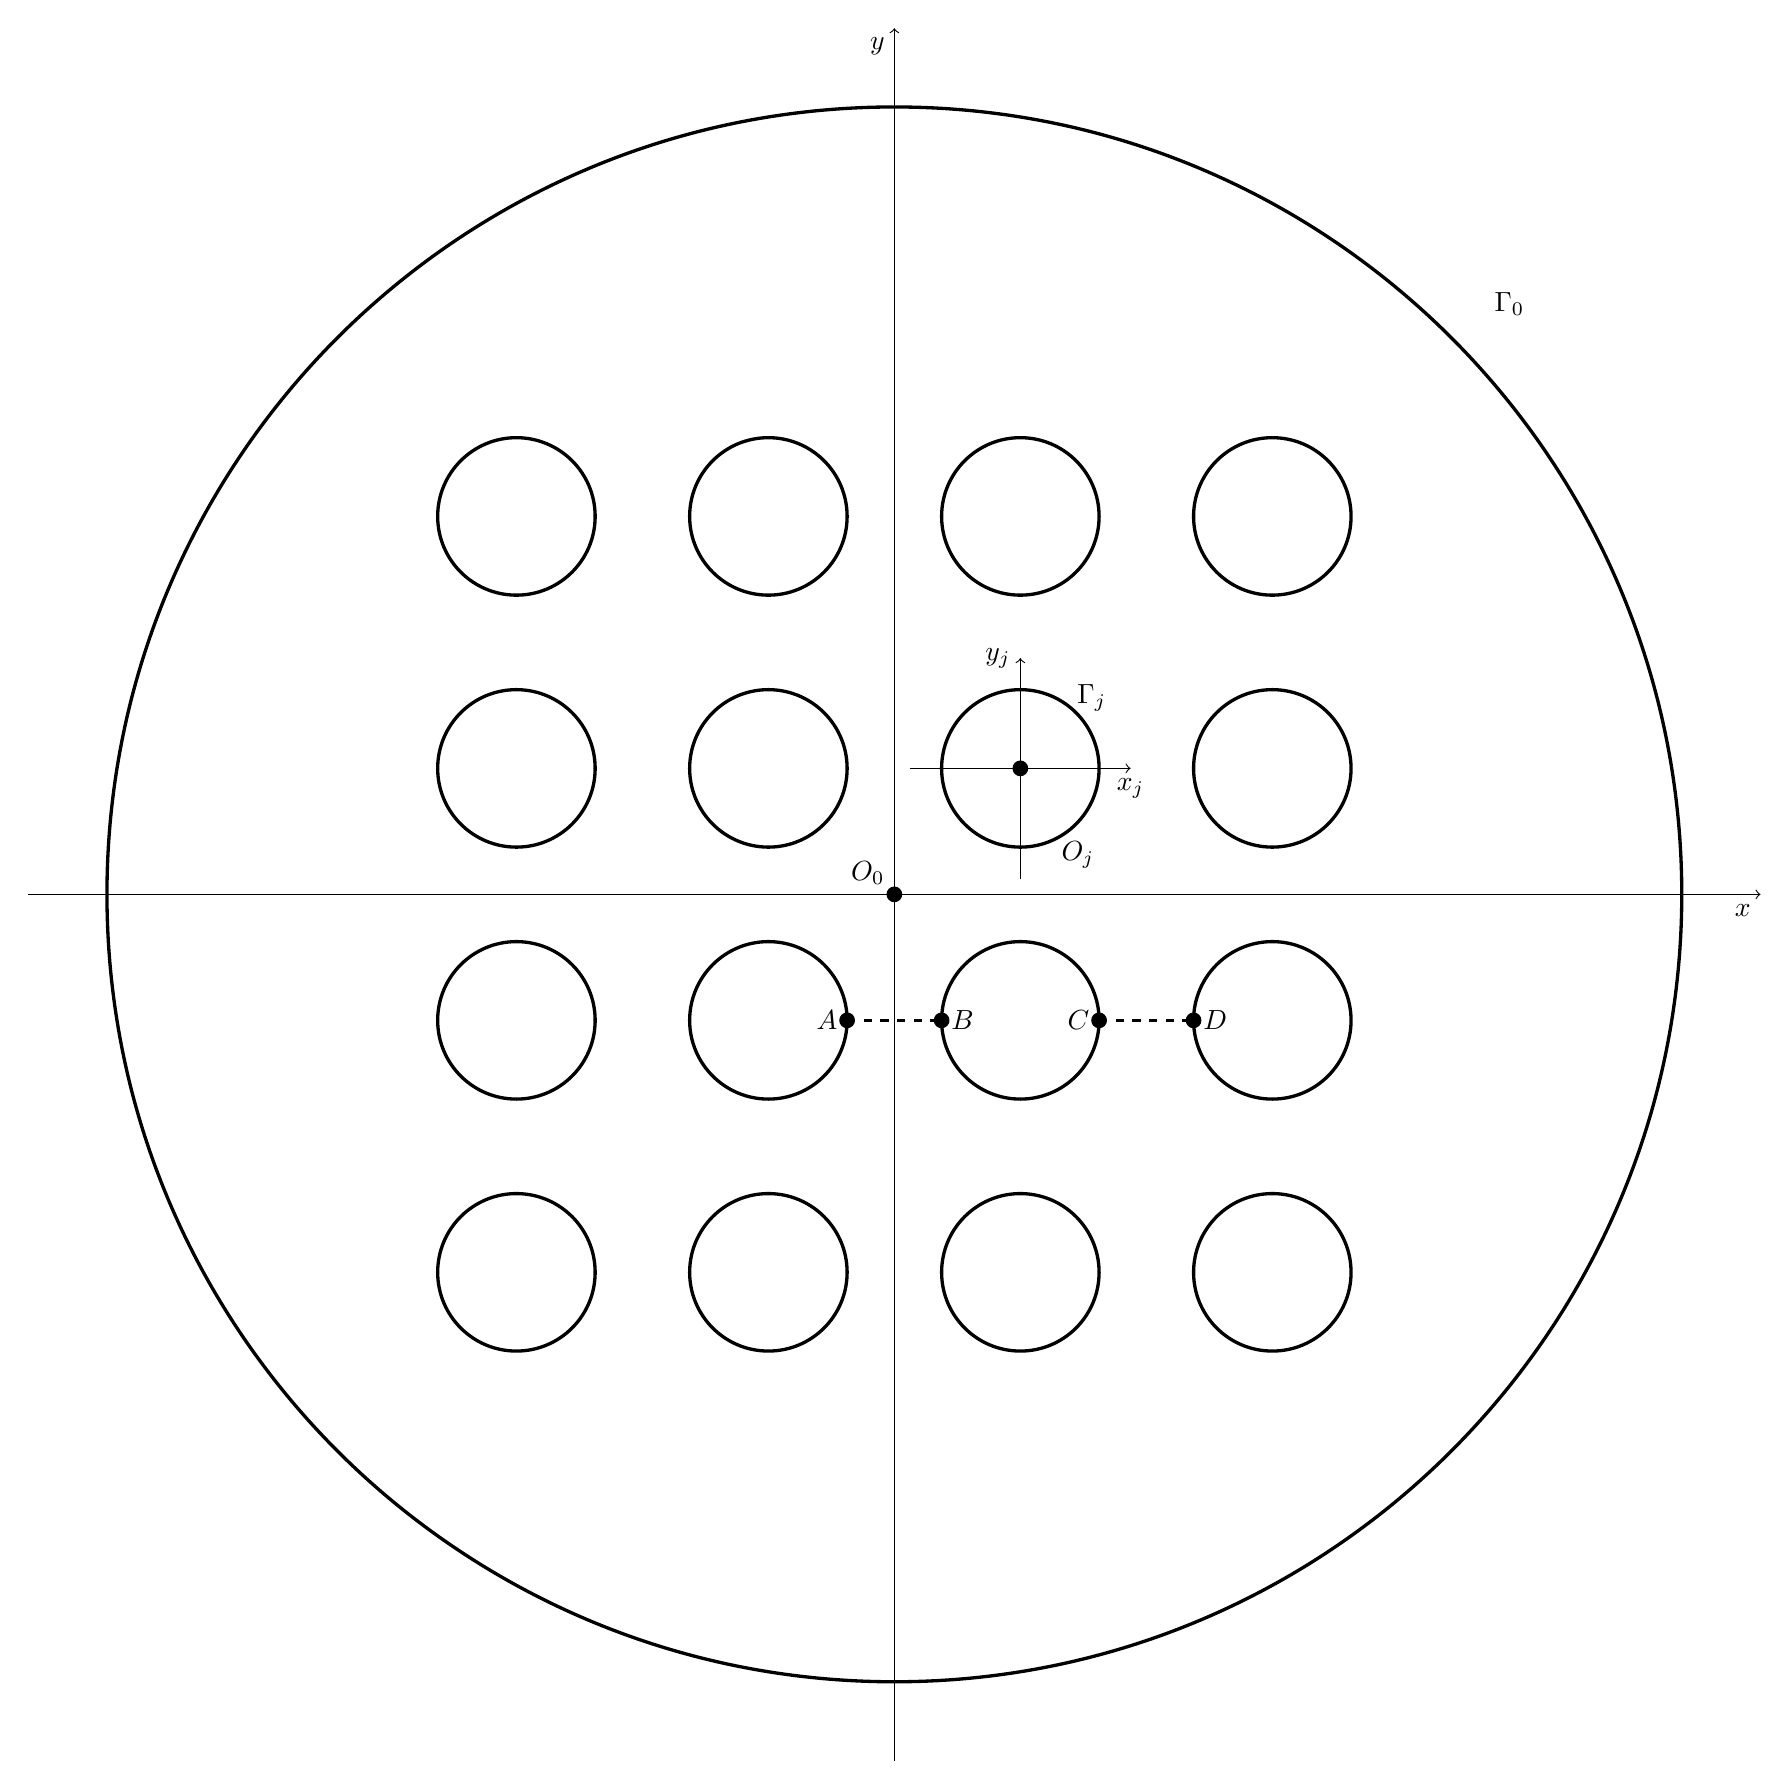
\begin{tikzpicture}
\coordinate (O) at (0,0);
\coordinate (O1) at (1.6,1.6);
\coordinate (O2) at (-1.6,1.6);
\coordinate (O3) at (-1.6,-1.6);
\coordinate (O4) at (1.6,-1.6);
\coordinate (O5) at (4.8,1.6);
\coordinate (O6) at (4.8,4.8);
\coordinate (O7) at (1.6,4.8);
\coordinate (O8) at (-1.6,4.8);
\coordinate (O9) at (-4.8,4.8);
\coordinate (O10) at (-4.8,1.6);
\coordinate (O11) at (-4.8,-1.6);
\coordinate (O12) at (-4.8,-4.8);
\coordinate (O13) at (-1.6,-4.8);
\coordinate (O14) at (1.6,-4.8);
\coordinate (O15) at (4.8,-4.8);
\coordinate (O16) at (4.8,-1.6);
\coordinate (A) at (-0.6,-1.6);
\coordinate (B) at (0.6,-1.6);
\coordinate (C) at (2.6,-1.6);
\coordinate (D) at (3.8,-1.6);

\draw[->] (-11,0) -- (11,0) node[below left] {$x$};
\draw[->] (0,-11) -- (0,11) node[below left] {$y$};

\draw[very thick] (O) circle (10.0);
\draw[very thick] (O1) circle (1.0);
\draw[very thick] (O2) circle (1.0);
\draw[very thick] (O3) circle (1.0);
\draw[very thick] (O4) circle (1.0);
\draw[very thick] (O5) circle (1.0);
\draw[very thick] (O6) circle (1.0);
\draw[very thick] (O7) circle (1.0);
\draw[very thick] (O8) circle (1.0);
\draw[very thick] (O9) circle (1.0);
\draw[very thick] (O10) circle (1.0);
\draw[very thick] (O11) circle (1.0);
\draw[very thick] (O12) circle (1.0);
\draw[very thick] (O13) circle (1.0);
\draw[very thick] (O14) circle (1.0);
\draw[very thick] (O15) circle (1.0);
\draw[very thick] (O16) circle (1.0);

%\fill[pattern=custom north west lines,hatchspread=8pt,hatchthickness=0.5pt,hatchcolor=black] (O1) circle(1.0);

\fill (O) circle(0.1) node[above left] {$O_0$};
\fill (O1) circle(0.1);
\fill (A) circle(0.1) node[left] {$A$};
\fill (B) circle(0.1) node[right] {$B$};
\draw[very thick, dashed] (A) -- (B);
\fill (C) circle(0.1) node[left] {$C$};
\fill (D) circle(0.1) node[right] {$D$};
\draw[very thick, dashed] (C) -- (D);

\node[right] at (2,0.5) {$O_j$};
\draw[->] (0.2,1.6) -- (3.0,1.6) node[below] {$x_j$};
\draw[->] (1.6,0.2) -- (1.6,3.0) node[left] {$y_j$};
\node[right] at (2.2,2.5) {$\Gamma_j$};
\node[right] at (7.5,7.5) {$\Gamma_0$};

\end{tikzpicture}
\end{document}

%%% Local Variables: 
%%% mode: latex
%%% TeX-master: t
%%% End: 
